\documentclass[12pt,a4paper]{article}

\usepackage[romanian]{babel}
\usepackage[utf8x]{inputenc}
\usepackage{amsmath}
\usepackage{graphicx}
\usepackage{gensymb}
\usepackage[colorinlistoftodos]{todonotes}
\usepackage{combelow}
\usepackage{newunicodechar}
\usepackage{url}

\newunicodechar{Ș}{\cb{S}}
\newunicodechar{ș}{\cb{s}}
\newunicodechar{Ț}{\cb{T}}
\newunicodechar{ț}{\cb{t}}
\newunicodechar{Ă}{\cb{A}}
\newunicodechar{ă}{\cb{a}}
\newunicodechar{Â}{\cb{A}}
\newunicodechar{â}{\cb{a}}
\newunicodechar{Î}{\cb{I}}
\newunicodechar{î}{\cb{i}}

\title{Inside NAV}
\author{Barcan Virgil-Gheorghe}

\begin{document}
\maketitle

\tableofcontents

\newpage
\section{Sistemul de operare Android}
\subsection{Despre Android \cite{AndroidHistoryAndroidCentral}} 
Android este un sistem de operare dedicat dispozitivelor mobile, smartphone-uri, smartwatch-uri, precum și TV-urilor sau chiar dispozitive din interiorul automobilelor.

Sistemul de operare Android este bazat pe un kernel de Linux și a fost construit pentru a fi folosit în principal pe dispozitive touchscreen. Este cel mai folosit sistem de operare disponibil pe dispozitive mobile încă din 2013.

Sistemul a fost dezvoltat de către Android Inc., companie fondată în 2003. Dezvoltatorii au avut dorința de a ajuta la construirea de dispozitive mai inteligente, conștiente de locația și preferințele utilizatorilor.

În 2005 compania Android Inc. a fost achiziționată de către Google pentru o sumă de aproximativ 50 milioane de dolari, iar intenția Google era clară pentru mulți, intrarea pe piața dispozitivelor mobile.

La data de 5 noiembrie 2007, un consorțiu de companii precum Google, HTC, Sony, Samsung, T-Mobile, dar și producători de chipset-uri, Qualcomm și Texas Instruments, a fost lansat. Acest consorțiu, numit „Open Handset Alliance”, al cărui scop era de a dezvolta standarde deschise pentru dispozitive mobile, a lansat în aceeași zi sistemul de operare Android, ca prim produs al său.

Primul smartphone cu sistem de operare Android lansat a fost HTC Dream, în luna octombrie a anului 2008.

Fiecare nouă versiune a sistemului este denumită în ordine alfabetică după un desert: „Cupcake”, „Donut”, „Eclair”, „Froyo”, „Gingerbread”, „Honeycomb”, „Ice Cream Sandwich”, „Jellybean”, „Kit Kat”, „Lolipop” și „Marshmallow”. Următoarea versiune este plănuită pentru acest an, deocamdată ea fiind denumită Android N. Google a oferit utilizatorilor posibilitatea să voteze numele.


\subsection{Versiunile Android \cite{AndroidVersionsHistory}, \cite{AndroidHistory}, \cite{DeveloperAndroid}}
\subsubsection{Android 1.0}
Prima versiune a sistemului de operare Android, denumită, deloc pompos, Android 1.0, dădea impresia de produs nefinalizat, însă lăsa să se întrevadă planurile Google pentru această platformă. Această versiune deja avea părți care, comparate cu ce era  pe piață la momentul acela, erau mult superioare. Sunt lucruri pe care acum le trecem cu vederea, dar care atunci erau noutăți, widget-urile, zonele de notificări și nu numai. 

Prima versiune a Android includea și aplicațiile cu care suntem acum atât de obișnuiți, cum ar fi Gmail sau YouTube. Android Market Beta debuta și ea, oferind posibilitatea de a lista aplicații și jocuri.

Tot în acea perioadă Android și-a câștigat și atât de cunoscutul logo, denumit în interiorul Google „Bugdroid”.


\subsubsection{Android 1.5 - Cupcake}
Primul mare update al Android-ului a fost versiunea 1.5, denumită, în ceea ce avea să stabilească trendul numelor inspirate din dulciuri, „Cupcake”.

	Lansat în aprilie 2009, Cupcake a fost deschizător de drum pentru dispozitivele cu Android fără tastatură fizică. Telefoanele precedente aveau încorporate și tastaturi fizice, însă cu această versiune de sistem de operare, Google a introdus tastatura virtuală, precum și posibilitatea folosirii de tastaturi third-party.

	Acestea arătau evenimentele și respectiv melodia curentă. Pentru prima dată aplicațiile puteau să își adauge widget-uri proprii. O altă noutate a fost reprezentată de posibilitatea de a roti automat ecranul în funcție de orientarea telefonului, pentru o tranziție ușoară portret-landscape.


\subsubsection{Android 1.6 - Donut}
În același an al lansării Android 1.5, Google a lansat și noua versiune, 1.6, numită „Donut”.
	
	Aceasta aducea suport pentru ecrane de diferite rezoluții și densități ale pixelilor, precum și suport nativ pentru comunicarea în banda CDMA (Code Division Multiple Access). Noul sistem oferea și posibilitatea de a efectua căutări, atât în fișierele aflate pe telefon, cât și pe internet, prin așa numitul „Quick Search Box”. Tot cu această versiune a venit și posibilitatea de a vedea consumul de baterie al dispozitivului.
	
	Android Market a fost refăcut pentru a putea expune aplicațiile gratuite de top, precum și aplicațiile de top plătite, în contextul exploziei de noi aplicații de pe această platformă. Pentru prima dată au fost introduse și butoane care ofereau acces facil la setări precum Wi-Fi, Bluetooth, GPS, Sincronizare sau Luminozitate.


\subsubsection{Android 2.0, 2.0.1, 2.1 - Eclair}
Lansat în octombrie 2009, Android 2.1, denumit și „Eclair”, a adus câteva îmbunătățiri precum: posibilitatea de a căuta în toate SMS-urile și MMS-urile salvate pe telefon, viteză de tastare mărită pentru tastatura virtuală, setări de accesibilitate, calendar, dar și un API pentru VPN (Virtual Private Network). Pentru browser, Android aducea suport HTML5. Tot acum au apărut double-tap-zoom și pinch-to-zoom.
	
	Tot în versiunea Eclair a fost introdusă și posibilitatea de a folosi Google Maps pentru navigație, aceasta oferind indicații pas-cu-pas, dar și informații legate de trafic, caracteristici similare serviciilor de navigație din automobile, cu diferența că cele oferite de Google erau gratuite.

	O altă funcționalitate care acum este extrem de utilizată și a fost adăugată înca din versiunea Eclair este cea de Speech-to-Text, care permitea introducerea de text dictând telefonului.
	

\subsubsection{Android 2.2 - Froyo}
Poate cea mai importantă noutate a acestei versiuni a fost aceea a introducerii mașinii virtuale Dalvik, care oferea Just-in-time Compiling, oferind îmbunătățiri masive ale vitezei Android-ului.

	Cu această versiune a fost oferită și posibilitatea de a instala sau muta aplicațiile pe cardul de memorie pentru a elibera memoria internă a telefonului. Altă noutate a fost reprezentată de hotspot-ul Wi-Fi, care permitea telefonului să ofere Wi-Fi altor dispozitive.

	Browser-ul a cunoscut și el îmbunătățiri ale vitezei prin schimbarea motorului de JavaScript la cel folosit de Chrome, V8.


\subsubsection{Android 2.3, 2.3.3 - Gingerbread}
Cu această nouă versiune a Android a apărut și ceea ce avea să devină un nou obicei al Google, acela de a lansa un telefon sub marcă proprie la câteva versiuni de soft distanță. Aceasă linie de telefoane se va numi Nexus și va fi construită cu producători diferiți la fiecare nouă iterație, ea oferind un Android „curat”. Primul telefon din gama Nexus a fost Nexus S, oferit de către Google în parteneriat cu Samsung.

	Sistemul de operare a adus suport pentru NFC (Near Field Communication), pentru ecrane cu rezoluții mari, pentru telefonie via internet (VoIP), dar și îmbunătățiri ale interfeței vizuale.

	Noul garbage collector concurent a adus un spor de viteză. A fost mărită și viteza de distribuție a evenimentelor în sistem. Tot cu această versiune s-a adăugat și suport nativ pentru mai mulți senzori (cum ar fi giroscopul și barometrul), suport pentru multiple camere video, dar și posibilitatea efectuării de apeluri video.

	Pentru dezvoltatori a fost îmbunătățit suportul pentru scrierea de cod nativ și s-au introdus API-urile pentru jocuri.


\subsubsection{Android 3.0 - Honeycomb}
Această nouă versiune a fost lansată cu scopul de a îmbunătăți experiența de utilizare a sistemului pe tablete. Pe lângă îmbunătățirile aduse la nivelul interfeței grafice, au fost aduse și îmbunătățiri la nivelul suportului pentru procesoare multi-core.

	A fost introdus și API-ul pentru utilizarea Fragmentelor, care permiteau dezvoltatorilor de aplicații sa folosească suprafața mai mare a ecranului unei tablete pentru a afișa mai multe părți ale aplicației. Folosirea Fragmentelor permitea separarea aplicațiilor pentru telefoane de cele pentru tablete într-un mod foarte simplu: dacă exista suficient spațiu, se afișau mai multe fragmente ale aplicației, altfel se afișa doar unul și utilizatorul trebuia să navigheze între acestea.

	A fost introdus și conceptul de Action Bar, adică acel spațiu din partea superioară a unei aplicații similar unui meniu dintr-o aplicație desktop.


\subsubsection{Android 4.0 - Ice Creak Sandwich}
Această versiune oferea o experiență unificată smartphone-tabletă, ea înlocuind complet versiunea Honeycomb și aducând noutățile ei și pe smartphone-uri.

	A fost îmbunătățit multitaskingul, notificările au devenit mai bogate, ecranul de start au fost și el modificat pentru a se reduce consumul de spațiu. S-a adăugat un sistem de management al consumului de date.

	Multitaskingul a devenit acum mai vizibil pentru utlizatorul final, acesta putând acum să selecteze aplicația pe care să o redeschidă. Utilizatorul poate vedea o listă de aplicații pe care le-a folosit în ultima perioadă, apoi poate selecta aplicația pe care să o readucă în prim-plan.

	În partea de jos a ecranului au apărut aplicațiile favorite, într-un aranjament similar celui de pe iPhone. Gesturile încep să devină parte esențială a experienței de utilizare a smartphone-ului, ele putând fi folosite pentru a șterge notificări, pentru a schimba tab-urile în browser, dar și pentru a respinge/accepta apeluri.

	Una din inovațiile aduse a fost Android Beam. Acest sistem permitea transferul de date între dispozitive care dispuneau de NFC. Acest transfer se făcea cu viteze mai mari decât ale Bluetooth-ului, într-un mod extrem de facil din perspectiva utilizatorului. Acesta trebuia doar să apropie cele două dispozitive și să apese „Trimitere”.


\subsubsection{Android 4.1, 4.2, 4.3 - Jelly Bean}
Această iterație a Android a adus noi îmbunătățiri la capitolul viteză prin introducerea „Project Butter”, care implementa Vsync și triple-buffering. Notificările au fost și ele modificate, putând conține acum până la 8 linii de text și chiar butoane la baza lor. Aceste butoane puteau fi folosite pentru a lua acțiuni în funcție de notificare.

	În Android Jelly Bean a fost lansat și Google Now, asistentul virtual al Google. Acesta oferă informații legate de vremea din locația curentă, precum și despre timpii necesari pentru a ajunge între diferite locații.

	Printre noutăți se numără și posiblitatea de a avea mai multe conturi pe același dispozitiv. Tot acum s-a adăugat și suportul pentru ecrane externe, eventual via Miracast (Wi-Fi Display).

	Alte îmbunătățiri sunt date de adăugarea HDR (High Dynamic Range), a Bluetooth Low Energy, dar și a OpenGL ES3.0, care aducea sporuri de performanță la nivel grafic.


\subsubsection{Android 4.4 - KitKat}
Poate cea mai importantă funcționalitate adăugată cu această versiune este cea a interacțiunii cu telefonul prin comenzi vocale. Faimosul „Ok, Google” a fost oferit începând cu această versiune. Tot acum s-au făcut eforturi pentru ca Android să poată rula mai bine pe dispozitive mai slabe din punct de vedere hardware. Acum Android putea rula chiar și pe 512 MB de RAM.

	S-a adăugat și un nou sistem de acces la stocare, care a permis dezvoltatorilor precum Box sau Dropbox să integreze serviciile lor direct cu memoria telefonului, oferind acces facil la documente din locații diferite.

	Au fost imbunătățiți și senzorii, prin reducerea consumului lor de baterie. Android nu  mai trimite notificările imediat cum senzorii observă modificările, ci le stochează până are suficiente.  Acum au fost introduși și senzorii de detectare a pașilor și de numărare a pașilor. 
	

\subsubsection{Android 5.0, 5.1 - Lollipop}
Android Lollipop a fost versiunea în care a apărut noul stil vizual propus de Google, „Material Design”. Acest ghid despre cum trebuie să arate interfața vizuală a aplicației a fost un mare pas către unificarea experienței de utilizare a aplicațiilor de pe această platformă.
	
	Material Design este un set de reguli de design inspirat din modul în care arată hârtia în diferite combinații de lumini și umbre.
Componentele grafice din aplicații erau acum reprezentate într-un mod minimalist, ca și cum ar fi niște colaje de hârtie. Google nu a adus doar recomandările legate de cum trebuie să arate componentele grafice, ci și un întreg set de instrumente noi care să ajute dezvoltatorii.
	
	Android 5.0 a adus și îmbunătățiri de performanță prin adăugarea ART runtime în locul Dalvik. Acum există suport pentru procesoare cu arhitectura pe 64 de biți. S-a adăugat suport pentru OpenGL ES 3.1, care a dus la jocuri mai bogate grafic și mai captivante.
	
	Tot începând cu această versiune Android și-a făcut apariția și în zona TV, prin lansarea Android TV. Android nu s-a oprit însă la zona TV, el apărând și în zona auto, prin Android Auto.

	
\subsubsection{Android 6.0 - Marshmallow}
Android Marshmallow a introdus un nou sistem de permisiuni pentru aplicații. Acest nou model presupunea ca aplicația să ceară drepturi de la utilizator nu la instalare, ci atunci când îi era necesar. Prin acest nou set de reguli se dorea ca utilizatorii să știe mai clar ce acceptă, deoarece înainte utilizatorii nu erau neapărat atenți la ce acceptau, și puteau exista aplicații care să poată avea acces la mai multe date decât le era necesar. Existau aplicații de genul „Lanternă” care aveau acces la contacte, locație, microfon și cameră. Genul acesta de permisiuni sunt în mod clar un pericol la intimitatea utilizatorilor, iar cu Android 6.0 Google a încercat să îl limiteze.

	O altă componentă a sistemului unde cei de la Google au adus îmbunătățiri este cea a consumului de baterie. Prin adăugarea „Doze” și a „App Standby”, aplicațiile consumă acum mai puțină baterie.

	În Marshmallow s-a adăugat și Now On Tap, un asistent virtual care permite să afli informații fără să părăsești aplicația curentă. Este util atunci când vrei să afli ce reprezintă ceva din aplicația curentă.


\subsubsection{Android N}
O nouă versiune a Android este în dezvoltare acum, aceasta având numele de cod „Android N”. Un nume care să urmeze linia numelor inspirate din produse dulci este în curs de a fi ales, Google oferind utilizatorilor posibilitatea să recomande și să voteze numele.
	
	Versiunea Android N este acum în developer preview. Aceast Android promite îmbunătățiri în 3 zone cheie: performanță, productivitate și securitate.
	
	Modificările nu se vor opri aici, ci vor include, pentru prima dată în Android, suport pentru mai multe ferestre. Android Instant Apps va permite testarea unor aplicații fără ca acestea să fie instalate efectiv pe dispozitiv.
	

\subsection{Senzorii disponibili pe platforma Android}
Majoritatea dispozitivelor care rulează Android au încorporați diverși senzori. Aceștia sunt folosiți în diferite contexte în timpul folosirii dispozitivului. Scopul senzorilor este să urmărească eventuale schimbări astfel încât sistemul să răspundă în cel mai bun mod cu putință.

	Deși poate nu este evident, impactul senzorilor este major. Faptul că ecranul se închide atunci când apropiem telefonul pentru a vorbi, faptul că putem să ne măsurăm distanțele parcurse, bătăile inimii, faptul că putem să folosim telefonul ca sistem de navigație, toate acestea se datorează folosirii senzorilor.
	
	Android împarte senzorii în mai multe categorii \cite{DeveloperAndroid}, deși tratarea lor se face într-un mod aproape unitar: senzori de \textbf{mișcare}, de \textbf{mediu}, de \textbf{poziție} și de \textbf{locație}.

	Încă un mod în care Android împarte senzorii este acela că senzorii pot fi \textbf{hardware} sau \textbf{software}.\\
	
\subsubsection{Sistemul de coordonate al senzorilor}
În general Android folosește un sistem de coordonate standard, cu 3 axe. Valorile venite de la senzori reprezintă schimbările pe aceste trei axe.

Sistemul de coordonate este definit în raport cu ecranul dispozitivului (ținut în pozitie verticală), astfel: axa $X$ este orizontală și orientată către dreapta, axa $Y$ este verticală si orientată către partea superioară a dispozitivului, iar axa $Z$ este axa care „iese” din centrul ecranului. Pentru o referință vizuală se poate consulta Figura \ref{fig:axis_device}, conformă cu documentația Android \cite{DeveloperAndroid}.

\begin{figure}[hbtp]
\centering
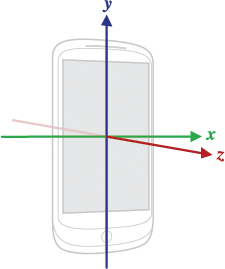
\includegraphics[width=5cm]{figures/axis_device.png}
\caption{Sistemul de coordonate}
\label{fig:axis_device}
\end{figure}


\subsubsection{Senzori de mișcare}
Acești senzori oferă posibilitatea monitorizării mișcării dispozitivului, de exemplu rotație, scuturare, înclinare sau legănare. Doi dintre acești senzori sunt mereu senzori fizici: \textbf{accelerometrul} și \textbf{giroscopul}. Ceilalți trei senzori pot fi atât hardware, cât și software: senzorul de \textbf{gravitație}, cel de \textbf{accelerație liniară} și \textbf{senzorul vectorului de rotație}. Recent au fost adăugați și senzori de \textbf{detectat}, respectiv \textbf{numărat pași}.

	\textbf{Accelerometrul} determină accelerația aplicată dispozitivului prin măsurarea forțelor aplicate senzorului în sine. Totuși, în aceste măsurători intră mereu în calcul gravitația.

	\textbf{Senzorul de gravitație} oferă un vector 3-dimensional care indică direcția și magnitudinea gravitației.

	\textbf{Senzorul de accelerație liniară} oferă un vector 3-dimensional care indică accelerația pe fiecare axă, excluând gravitația.

	Putem formaliza relația dintre accelerații astfel:
	$A_{liniara} = A - g$.\\

	\textbf{Giroscopul} măsoară viteza angulară în raport cu axele $X$, $Y$, $Z$. Viteza angulară este măsurată în $rad/sec$.\\

	\textbf{Senzorul vectorului de rotație} reprezintă orientarea dispozitivului ca fiind combinația dintre o axă și un unghi. Dispozitivul este rotit în jurul uneia dintre axele $X$, $Y$, $Z$ cu un unghi $\theta$. Cele trei componente ale vectorului de rotație sunt: $(x \sin{\theta}, y \sin{\theta}, z \sin{\theta})$. 
	
	Comparativ cu ceilalți senzori de mișcare, acest senzor are valorile exprimate într-un alt sistem de coordonate, unul „global”.
	Acest sistem are următoarele caracteristici:
	\begin{itemize}
	\item $X$ este definit ca fiind tangent la pământ în locația curentă și orientat către Est,
	\item $Y$ este definit ca fiind tangent la pământ în locația curentă și orientat către Polul Nord Magnetic,
	\item $Z$ este definit ca fiind perpendicular la planul definit de $X$ și $Y$, orientat către cer.
	\end{itemize}
	
	Referința vizuală a acestei descrieri este în Figura \ref{fig:axis_globe}, conformă cu documentația Android \cite{DeveloperAndroid}.

\begin{figure}[h]
\centering
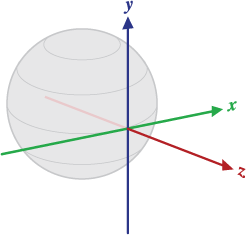
\includegraphics[width=5cm]{figures/axis_globe.png}
\caption{Sistemul de coordonate utilizat de senzorul vector de rotație}
\label{fig:axis_globe}
\end{figure}

\subsubsection{Senzori de mediu}
Acești senzori permit monitorizarea unor valori precum \textbf{umiditatea}, \textbf{intensitatea luminoasă}, \textbf{presiunea atmosferică} sau \textbf{temperatura mediului} din apropierea dispozitivului. Toți senzorii menționați sunt hardware.

Senzorii de \textbf{intensitate luminoasă}, \textbf{presiune atmosferică} sau \textbf{temperatură} sunt unii dintre cei mai simplu de utilizat deoarece nu este necesar ca datele lor să fie corectate. Ei oferă valori cu următoarele unități de măsură: $lx$ (lux) pentru intensitatea luminoasă, $mbar$ (milibar) pentru presiunea atmosferică, respectiv $\celsius$ (grade Celsius) pentru temperatură.

Senzorul de \textbf{umiditate} este și el simplu de folosit. Valorile oferite de el sunt procente.


\subsubsection{Senzori de poziție}
Acești senzori permit monitorizarea poziției dispozitivului într-un cadru de referință global, prin urmărirea schimbărilor de \textbf{câmp magnetic} sau a \textbf{orientării}. Un alt senzor care face parte din această categorie este și  \textbf{senzorul de proximitate}.

\textbf{Senzorul de câmp magnetic} arată fluctuațiile câmpului magnetic al Pământului pe cele trei axe. El oferă valori a căror unitate de măsură este $\mu$T (microTesla). În mod uzual datele de la acest senzor nu sunt folosite în forma lor brută, ci în combinație cu alte date. De exemplu, datele sale, împreună cu cele venite de la accelerometru, pot fi folosite pentru a obține matricile de rotație și de înclinație. Aceste matrici pot fi foloste pentru a se obține \textbf{azimutul}. Azimutul este unghiul la care suntem față de Polul Nord Magnetic. După declinarea magnetică acest unghi ajunge să arate diferența față de Polul Nord, acționând similar unei busole.

\textbf{Senzorul de orientare} permite monitorizarea poziției relative a dispozitivului în raport cu sistemul de coordonate global. Acest senzor face fuziunea descrisă mai sus, combinând datele de la magnetometru și de la accelerometru pentru a obține \textbf{azimutul} (gradele de rotație în jurul axei $Z$), \textbf{pitch}-ul (gradele de rotație în jurul axei $X$) și \textbf{roll}-ul (gradele de rotație în jurul axei $Y$). Deoarece combinarea datelor de la ceilalți doi senzori consumă foarte mult, precizia senzorului este diminuată. De aceea, acest senzor a fost declarat depășit și Android recomandă utilizarea metodei prezentate mai sus pentru obținerea orientării (via matricile de rotație și înclinație).

\textbf{Senzorul de proximitate} raportează cand telefonul este „aproape” sau „departe” de un alt obiect. În mod uzual distanța începând cu care un obiect este considerat apropiat/depărtat este de 5 $cm$.

\subsubsection{Senzori de locație}
Acești senori primesc date despre locația curentă a dispozitivului. Locația curentă poate fi obținută din mai multe surse, cu erori mai mici sau mai mari. Printre surse numim: \textbf{GPS}-ul, \textbf{Wi-Fi}-ul sau chiar datele de \textbf{celulă telefonică}. Pe lângă erorile ce pot veni din faptul că avem de a face cu multiple surse, nici datele provenite din aceeași sursă nu sunt cele mai precise.

Android oferă aplicațiilor acces la servicii de localizare în funcție de ce este disponibil pe dispozitiv. API-ul pentru locație este puțin diferit față de cel pentru ceilalți senzori.\\

Deși acești senzori sunt recunoscuți de către Android, nu este obligatoriu ca toți să fie prezenți și pe dispozitiv. Android nu impune ce senzori să fie prezenți pe dispozitive, ei doar recomandă prezența unora de bază pentru o utilizare cât mai apropiată de cea normală. Producătorii de dispozitive pot la fel de bine să mai adauge senzori noi, nici acest lucru nu este îngrădit de modul de lucru al Android. Fiind open-source, i se poate adăuga suport destul de ușor pentru senzori noi.


\section{Obiecte Android}
Sistemul de operare Android oferă o platformă bogată pentru a permite dezvoltarea de aplicații. Aplicațiile Android sunt scrise în Java. Pe lângă \textbf{Java}, se poate utiliza și \textbf{C++}, prin includerea \textbf{NDK} (Native Development Kit).

Modul în care aplicațiile Android sunt structurate diferă comparativ cu modul „uzual” (al aplicațiilor desktop). Aplicațiile sunt alcătuite din mai multe componente: \textbf{activități}, \textbf{servicii}, \textbf{content provider}, \textbf{broadcast receiver}, fiecare dintre ele putând fi invocată în orice moment. Astfel aplicațiile pot avea mai multe puncte de intrare, câte unul pentru fiecare activitate componentă.

Comunicarea între aceste componente se face folosind alte obiecte specifice Android, \textbf{intent}-urile. Un intent este modul prin care o componentă „spune” ce dorește să facă: să pornească o altă componentă, să ceară deschiderea aplicației standard pentru a afișa conținut, să transmită parametri și nu numai.

O altă componentă esențială a unei aplicații Android este \textbf{manifestul}. Acest fișier XML este folosit pentru a descrie ce componentă trebuie pornită prima dată, care sunt componentele aplicației, ce permisiuni cere aplicația, care este API-ul minim suportat de aplicație, descrie funcționalități hardware sau software pe care aplicația le folosește (acces la Bluetooth, la cameră, etc.)

Pentru stocarea de date Android oferă posibilitatea folosirii unor obiecte de sistem numite \textbf{SharedPreferences}. Acestea stochează datele într-un format XML, similar unui dicționar dintr-un limbaj de programare, în modul cheie-valoare. Pe lângă SharedPreferences se mai pot utiliza și bazele de date SQLite sau fișiere pe stocarea dispozitivului.

Înainte de a continua cu explicarea fiecărei componente, vom descrie succint cum se construiește și cum se rulează o aplicație. Pentru a construi o aplicație, Android pune la dispoziție unelte prin \textbf{SDK} (Software Development Kit). Aplicațiile sunt construite într-un \textbf{pachet Android} a cărei extensie este .apk. Un .apk conține tot ce este necesar aplicației pentru a rula. Fiecare aplicație rulează în izolare, în propria sa mașină virtuală. Fiecare aplicație rulează ca un proces Linux. Android pornește acest proces atunci când se cere deschiderea aplicației și îl închide atunci când fie utilizatorul închide aplicația, fie sistemul are nevoie de resursele consumate de aplicație și aceasta nu este folosită.

\subsection{Componentele unei aplicații}
Așa cum am amintit deja, există patru tipuri de componente: \textbf{activități}, \textbf{servicii}, \textbf{content provider}, \textbf{broadcast receiver}.

\subsubsection{Activități}
O activitate este o componentă a unei aplicații care oferă un ecran prin care utilizatorul să interacționeze cu ea. Fiecare activitate primește o fereastră pe care să deseneze elementele sale grafice.

Pentru a crea o activitate este necesar să fie creată o clasă care să extindă clasa de bază Activity. Prin aceasta ni se va cere să implementăm metoda onCreate(). Această metodă este entry-point-ul în activitate, similar unui main().

Pentru a trata diferite situații posibile în ciclul de viață al activității este necesar să implementăm metode de tip callback prin care Android să ne notifice. Astfel putem primi notificare când suntem opriți, cand am fost readuși în focus, etc. Ciclul de viață al unei activități este prezentat în Figura \ref{fig:activity_lifecycle}, așa cum apare ea în documentația Android \cite{DeveloperAndroid}.

\begin{figure}[h]
\centering
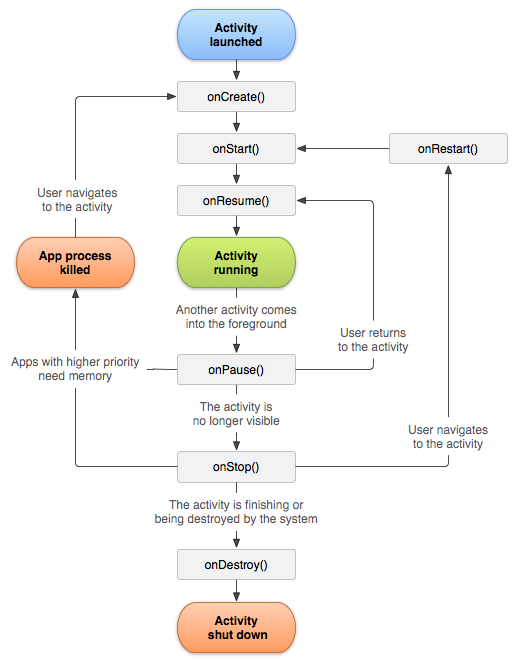
\includegraphics[width=10cm]{figures/activity_lifecycle.png}
\caption{Ciclul de viață al unei activități}
\label{fig:activity_lifecycle}
\end{figure}

Fiind componente prin care utilizatorul poate interacționa cu aplicația, o activitate trebuie să ofere un layout în care să își declare componentele grafice. Acest lucru se face prin scrierea unui XML în care să fie descrisă structura elementelor. Există mai multe modalități de așezare a elementelor grafice pe ecran, iar acestea poartă numele de layout-uri. Amintim: LinearLayout, RelativeLayout, GridLayout, CardLayout, dintre cele mai folosite. Pe lângă layout, este necesar să adăugăm și componente precum butoane sau input-uri. Android are o paletă largă de astfel de elemente, iar unde biblioteca standard nu are elemente se poate interveni fie cu cod propriu, fie cu biblioteci externe.

Dacă se dorește un mod de afișare mai dinamic, se pot adăuga \textbf{Fragmente}.

Un \textbf{Fragment} reprezintă o componentă modulară a unei activități. O activitate poate conține mai multe fragmente care să interacționeze între ele. Este ca și cum am construi o aplicație desktop cu mai multe ferestre disponibile, doar că aici nu avem ferestre efective, ci zone din activitate. Activitatea descrie în layout unde trebuie așezat fiecare fragment iar apoi poate modifica din cod așezarea acestora pentru a crea un comportament dinamic. Putem avea pe o aceeași activitate două ecrane și să ajungem de la unul la celalalt printr-un swipe.

Marele avantaj al fragmentelor este acela că oferă funcționalități similare din punctul de vedere al utilizatorului cu o activitate, însă totul în interiorul unei activități, ceea ce scutește sistemul de la un efort suplimentar. Interfețele devin mai rapide și mai fluide, pe lângă marele avantaj al oferirii unei experiențe mai plăcute pentru utilizator.

\subsubsection{Servicii}
Serviciile sunt componente ale aplicației care pot efectua operații în fundal (nu au o parte care să interacționeze cu utilizatorul, așa cum au activitățile). Serviciile sunt utile pentru operații de genul citire fișiere mari, interacțiune cu senzori, interacțiune cu rețeaua.

Un serviciu poate lua două forme: \textbf{pornit} sau \textbf{„lipit”}. Un serviciu pornit poate rula în fundal pentru o perioadă nedeterminată de timp, chiar dacă acea componentă care l-a pornit a fost distrusă. Serviciul se va opri singur atunci când își finalizează treaba. Un serviciu „lipit” este acel serviciu care oferă o interacțiune de tip client-server cu acea componentă care l-a pornit. Dacă oprim componenta care a pornit serviciul, se oprește și serviciul.

Pentru a crea un serviciu este necesar să fie creată o clasă care să extindă clasa Service. La fel ca în cazul activităților, Android ne va anunța prin callback-uri când se întâmplă evenimente relevante. Ciclul de viață al unui serviciu este prezentat în Figura \ref{fig:service_lifecycle}, așa cum apare ea în documentația Android \cite{DeveloperAndroid}.

\begin{figure}[h]
\centering
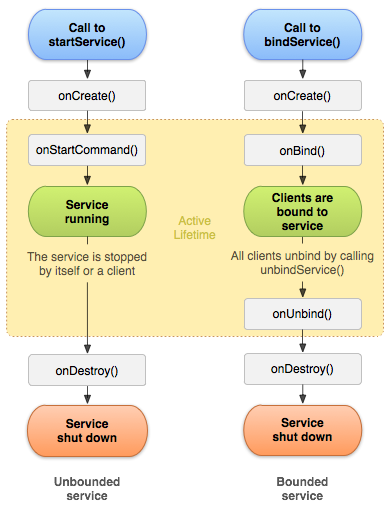
\includegraphics[width=10cm]{figures/service_lifecycle.png}
\caption{Ciclul de viață al unui serviciu}
\label{fig:service_lifecycle}
\end{figure}

\subsubsection{Content Provider}
Un content provider este o componentă care oferă acces la un set de date structurate, cum ar fi, de exemplu, contactele. Aceste componente încapsulează datele și oferă mecanisme pentru a defini chestiuni de securitate. Utilizarea lor este atunci când se dorește să se ofere acces la datele oferite de un proces unui alt proces.
Modul de lucru cu această componentă este similar într-o oarecare măsură cu lucrul cu o bază de date. Pentru a primi date se fac interogări, iar pentru a parcurge datele folosim un cursor.

\subsubsection{Broadcast Receiver}
Un broadcast receiver este o componentă care permite captarea și procesarea unor mesaje trimise de tip broadcast, trimise către oricine le poate înțelege și procesa.

Această componentă este declarată în AndroidManifest, acolo unde se specifică și ce mesaje poate să înțeleagă. Utilitatea lor este, de exemplu, de a „asculta” când s-a repornit telefonul, eventual pentru a porni alte aplicații și servicii.


\subsection{API-uri Google}
Pe lângă paleta largă de obiecte pe care o pune la dispoziție prin sistemul Android, Google mai oferă și acces la servicii suplimentare care pot aduce mari îmbunătățiri aplicațiilor. Sunt servicii care scutesc dezvoltatorii de scris și testat cod, oferindu-le metode de a afișa hărți, de a introduce componente sociale în aplicații, de a construi jocuri noi, de a face procesări în cloud și nu numai.

Deși există o gamă largă de API-uri disponibile, vom discuta pe scurt doar despre unul dintre acestea, relevant în contextul acestei lucrări, Google Maps API.

\subsubsection{Google Maps API \cite{GoogleMapsAndroidAPI}}
API-ul Google Maps oferă dezvoltatorilor posibilitatea adăugării de hărți în aplicațiile lor. Aceste hărți pot conține toate funcționalitățile pe care le găsim în aplicația Google Maps, printre care și clădiri 3D, hărți ale clădirilor, imagini din satelit.

API-ul se ocupă în mod automat de tot ce înseamnă comunicarea cu serverele Google și cu afișarea hărții. Dezvoltatorul trebuie doar să implementeze funcționalitățile dorite peste cele de bază oferite deja de Google Maps. Dezvoltatorul poate, spre exemplu, să adauge propriul design harților, să modifice unghiul de vizualizare, să adauge linii, puncte sau alte elemente grafice pe diferite nivele (layers).


\newpage
\section{Aplicații și cercetări similare existente}
Domeniul navigației cu ajutorul senzorilor este unul în care se fac studii intense datorită impactului pe care îl poate avea. Putem găsi utilizări în industrii precum cea automotive, în zona de vânzări produse, în zona medicală sau ca ajutor pentru echipe de salvare.

În studiul pentru elaborarea acestei lucrări am citit studii precedente, axate pe diferite componente ale aplicației pe care vreau să o dezvolt. Sunt cercetări în zona detecției pașilor cât mai corect, în zona determinării lungimii parcurse cu fiecare pas sau chiar în partea de hărți și orientare.

Pe lângă studiile citite, am încercat să găsesc și aplicații similare cu care să compar munca mea. Aceste aplicații mi-au oferit, pe lângă posibilitatea de a mă compara cu ceva, și idei pe care să la folosesc în propria implementare.

O să încep cu cercetările existente deoarece consider că acestea stau la baza ulterioarelor dezvoltări de aplicații.

\subsection{Cercetări similare existente}
Dacă este să analizăm munca de cercetare făcută, a cărei rezultat nu a fost o aplicație publicată, trebuie să luăm în considerare câteva articole care explică diferite metode de a obține ce se dorește și prin această lucrare.

Aceste articole au fost publicate de echipe întregi, cu acces la finanțare și la tehnică. Acele articole care nu au fost făcute în echipă au fost făcute ca lucrări de master sau chiar de doctorat. %TODO: Modificare daca nu e asa%

Dintre sursele pe care le consider relevante și de la care am învățat vreau să enumăr:
 
\begin{itemize}  
\item \textbf{Dead Reckoning Algorithms for Indoor Localization} \cite{ZhangYu}:\\
Această lucrare este teza de masterat a singaporezului Zhang Yu și a reprezentat un punct de sprijin în elaborarea lucrării mele, atât prin informațiile oferite de el, cât și prin bibliografia extinsă pe care a prezentat-o. În bibliografia lui am găsit alte articole extrem de interesante din care am luat idei.

În teza sa de master, el a încercat să compare robustețea unui număr de algoritmi de dead reckoning pentru persoane, folosind senzorii unei tablete. Diferența este că el face procesarea offline, nu pe dispozitiv. Aplicația pe care eu doresc să o propun face procesarea în timp real.

Algoritmii prezentați de acesta variază de la algoritmi bazați pe \textbf{triangularizare folosind Wi-Fi} până la \textbf{Filtre Kalman Extinse}. Este de interes și studiul capabilităților senzorilor făcut de către Zhang Yu. De asemenea, principiile detecției pașilor au fost de mare ajutor.

\item \textbf{A Step, Stride and Heading Determination for the Pedestrian
Navigation System} \cite{StepLengthAndHeadingDetermination}:\\
Această lucrare prezintă principiile de bază ale detecției pașilor, determinării lungimii unui pas și a orientării. Este o lucrare cu o analiză destul de detaliată a mersului uman, din care se extrag metode experimentale de determinare a pașilor.

\item \textbf{Using the ADXL202 in Pedometer and Personal Navigation Applications} \cite{HarveyWeinberg}:\\
Acest scurt articol prezintă o formulă de calculare a distanței parcurse într-un pas.

Formula estimează lungimea unui pas k, $\rho_{k}$, ca fiind $\rho_{k} = K \sqrt[4]{A_{max}^{(k)} + A_{min}^{(k)}}$, unde $A_{max}^{(k)}$ este valoarea maximă a accelerației în timpul celui de-al k-lea pas, $A_{min}^{(k)}$ este valoarea minimă a accelerației în timpul celui de-al k-lea pas, iar $K$ este o constantă dependentă de utilizator. Această constantă se va afla printr-o procedură de calibrare.

Această formulă este ulterior demonstrată ca fiind una bună în practică de către Diego Alvarez și colegii săi în articolul „Comparison of step length estimators from wearable accelerometer devices” \cite{StepLengthEstimatorsComparaison}.

\item \textbf{An Indoor Navigation System For Smartphones} \cite{AbhijitChandgadkar}:\\
În această lucrare se prezintă o modalitate de a oferi navigație în interiorul clădirilor, similar lucrării noastre. Aceasta se bazează pe aceeași idee de a estima poziția pe baza distanței parcurse cu fiecare pas și a diferențelor de orientare. 

Se introduce și o metodă de reducere a erorilor prin folosirea unor marcaje amplasate în puncte cheie ale clădirii. Pentru aplicația noastră nu este fezabil un plan similar deoarece nu există o clădire țintă, ci se dorește funcționarea în orice clădire.

\item \textbf{Exploring Smartphone-Based Indoor Navigation: A QR Code Assistance-Based Approach} \cite{QRNavigation}:\\
În acest articol este prezentată o metodă de navigație similară celei implementate în această lucrare. 

Pentru reducerea erorilor autorii propun montarea unor marcaje cu coduri \textbf{QR} (Quick Response) în puncte cheie ale clădirii. La fel ca mai sus, nu este fezabilă o astfel de abordare decât atunci când există clădiri țintă în care aplicația va fi folosită.

\item \textbf{Filtering and Tracking for a Pedestrian Dead-Reckoning System} \cite{SuratKwanmuang}:\\
În această lucrare de doctorat se implementează un sistem capabil să urmărească mișcările unui om pentru ca mai apoi un robot să poată urma o aceeași traiectorie. Motivația din spatele acestei idei este aceea de a avea un robot care să care provizii sau materiale grele în locul omului. Această aplicație are potențiale implicații în zona militară.

Deși se implementează un dead reckoning pe bază de filtru Kalman, aplicația are un mare dezavantaj, acela că limitează utilizatorul la purtarea senzorului fixat pe picior. Această limitare face ca aplicația să nu fie utilă în zona în care dorește să intre aplicația prezentată în această lucrare de licență, aceea de a avea navigație pe dispozitive deja disponibile, fără a fi nevoie de alți senzori.

\item \textbf{Filtering and Tracking for a Pedestrian Dead-Reckoning System} \cite{SDCPA10b} și \textbf{Indoor pedestrian navigation system using a modern smartphone} \cite{SCM10}:\\
Aceste articole stau la baza implementării unei aplicații la \textbf{CRS4} (Center for Advanced Studies, Research and Development in Sardinia) a unei aplicații, \textbf{Roodin}. Această aplicație are la bază o idee similară aplicației prezentate în această licență.

\item \textbf{Pedestrian localisation for indoor environments} \cite{OliverWoodman}:\\
În teza sa de doctorat, Oliver Woodman prezintă metode de a obține navigație în interiorul clădirilor folosind senzori. Explicațiile sale cu privire la senzori și la ce înseamnă un sistem de navigație inerțială sunt importante pentru a înțelege eventualele surse de eroare.

Prezentarea sa ajunge la disuții privitoare la filtre posibile care să îmbunătățească acuratețea (cum ar fi filtre Bayes sau filtre Kalman). Ideile prezentate de către el pot reprezenta un eventual punct de plecare pentru ulterioare îmbunătățiri ale aplicației prezentate.

Totuși, implementarea sa se bazează pe folosirea unor senzori externi, montați pe picior, ceea ce limitează aplicabilitatea sa.

\end{itemize}


\subsection{Aplicații similare existente}
În încercarea de a oferi sisteme de navigație rezistene la erori sau la lipsa semnalului s-au construit mai multe aplicații similare cu cea din această lucrare.

Aceste aplicații fie încearcă îmbunătățirea semnalului GPS prin adăugarea măsurătorilor de la senzori, fie încearcă să ofere posibilitatea navigării exclusiv folosind senzorii, fie ei senzorii descriși în unul din capitolele anterioare, fie ei camera telefonului sau chiar Wi-Fi-ul.

Am putea considera aplicații similare și acele aplicații care încearcă oferirea de noi informații utilizatorilor folosind date de la GPS și senzori, de exemplu pentru a găsi poziția și respectiv orientarea lor în raport cu eventuale puncte de interes.

\begin{itemize}  
\item \textbf{Google Maps} \cite{GoogleMaps}:\\
Dacă discutăm despre aplicații despre navigație pentru pietoni, nu putem omite poate cea mai cunoscută dintre ele, Google Maps. Această aplicație este oferită de către Google și oferă funcționalități de bază, cum ar fi afișarea locației curente, oferirea de indicații către alte locații, dar și afișarea de informații legate de mijloacele de transport în comun sau starea traficului. Este o aplicație care arată cât de multe date are Google la dispoziție. 

Marele dezavantaj al acestei aplicații este acela că are nevoie de acces la semnal GPS și la serviciul de date pentru descărcarea hărților (se oferă acum posibilitatea descărcării hărților pentru ca aplicația să funcționeze și offline).
 
Google Maps este inutil în zonele cu semnal GPS slab sau în interiorul clădirilor. Nu îl putem folosi, de exemplu, pentru a găsi o sală de curs într-o facultate, un cabinet într-un spital sau un magazin într-un mall. 
 
\item \textbf{Strava} \cite{Strava}:\\
O altă aplicație care oferă navigație pentru pietoni, și nu numai, este Strava. Această aplicație a fost construită ca un asistent de fitnes folosit pentru a înregistra traseele celor cărora le place să facă sport, însă componenta sa socială permite salvarea de trasee și oferirea/parcurgerea lor.

Deoarece este în principal o aplicație de fitness, Strava nu pune mare accent pe parte de navigație. Nu găsim în Strava informațiile pe care le găsim în Google Maps. Pe lângă acest dezavantaj, și Strava suferă de aceeași problemă a dependenței de GPS. Fără GPS aplicația doar măsoară numărul de pași și estimeasă distanța parcursă.

\item \textbf{SmartNavi - Step Navigation} \cite{SmartNavi}:\\
O aplicație care se apropie de ceea ce se dorește a fi această lucrare este SmartNavi - Step Navigation. Această aplicație a fost creată în cadrul unui set de experimente pentru platforma Android, prin care Google a oferit posibilitatea unor dezvoltatori să își pună ideile în practică, aceștia beneficiind de marketingul făcut de compania gigant. Prin participarea la aceste experimente, dezvoltatorii sunt de acord să facă public codul sursă pentru a putea fi folosit și de către alți dezvoltatori care să ducă mai departe ideile și să lanseze aplicații noi.

Aplicația oferă posibilitatea de a oferi navigație fără a avea semnal GPS, doar pe baza măsurării numărului de pași și a direcției luate de utilizator. Aceste este un mare avantaj dacă o comparăm cu aplicații precum Google Maps sau Strava. Aplicația recunoaște pașii și direcția bazându-se pe senzorii dispozitivului. 

Pe lângă oferirea de navigație, aplicația poate să se comporte ca un furnizor de locație, care poate fi util pentru alte aplicații din sistem. 

Dezavantajul acestei aplicații este că utilizatorul trebuie să țină mereu telefonul în fața lui (deși poziția este una normală pentru situația în care trebuie să urmărească indicațiile de pe ecran, pot exista situații în care utilizatorul să dorească să țină telefonul în altă poziție).

SmartNavi dorește să ofere posibilitatea de a avea navigație fără un consum foarte mare de baterie, dorința lor nu este neapărat de a oferi un sistem capabil de a lucra în interiorul clădirilor. Acesta poate fi privit ca un dezavantaj, aplicația nu are o țintă clară, ea doar dorește să arate ce este posibil pe această platformă.

\item \textbf{DaRe - Pedestrian Navigation} \cite{DaRe}:\\
Aplicația DaRe oferă navigație primind date de la un senzor montat pe piciorul purtătorului, care comunică prin Bluetooth cu smartphone-ul. DaRe are două moduri de lucru: metoda grafică, în care afișează traseul pe un plan bi-dimensional, și modul text, în care afișează date cum ar fi: numărul de pași, distanța parcursă și viteza medie. 

Totuși, comparativ cu aplicația descrisă în această lucrare, DaRe are marele avantaj de a avea un senzor extern plasat exact pe piciorul purtătorului. Asta garantează că pașii vor fi detectați aproape perfect, comparativ cu detecția făcută cu ajutorul telefonului. Măsuratorile făcute cu telefonul sunt predispuse la mișcările utilizatorului, care pot să declanșeze detectorul de pași și să numere în plus.

Un alt dezavantaj al DaRe este acela că nu plasează utilizatorul pe o hartă, ci doar îl arată într-un plan bidimensional simplu. Aplicația nu are decât scop de testare al posibilităților unui astfel de sistem.

\item \textbf{Landmarker} \cite{Landmarker}:\\
O altă aplicație care se bazează foarte mult pe senzori și pe locație pentru a oferi utilizatorului informații este Landmarker. Această aplicație dorește să aducă pe platforma Android un mod nou de a găsi puncte de interes în orașe. 

Aplicația recunoaște poziția curentă a utilizatorului și, folosind senzorii dispozitivului, reacționează la mișcările acestuia, arătându-i pe ecran unde (distanța și punctul cardinal) se află locațiile de interes.

Landmarker intră într-o altă zonă față de toate celelalte aplicații, aceea a oferirii de informații legate de puncte de interes din apropiere. Nu se ocupă de oferirea de navigație (ba chiar oferă posibilitatea să se treacă la Google Maps dacă se dorește a se găsi un traseu până la punctul de interes) și este dependentă de GPS. Este interesantă în contextul lucrării curente deoarece folosește senzorii telefonului pentru a determina orientarea față de un punct cardinal, ceea ce este esențial pentru oferirea de navigație în clădiri sau zone cu semnal GPS slab.

\item \textbf{Maps People} \cite{MapsPeople}:\\
Aceast serviciu oferă componenta lipsă a oricărei aplicații de navigație în interiorul clădirilor, adică partea de hărți. Este un serviciu cu plată care permite căutarea de locații, oferirea de anunțuri relevante și de rute între locații.

\end{itemize}

\newpage
\section{Motivație}
Problema pe care încerc să o rezolv prin această lucrare de licență este să ofer un sistem robust de navigație, indiferent de mediul în care telefonul este folosit.

La momentul actual Android este cel mai utilizat sistem de operare pentru dispozitive mobile, iar acest fapt poate avea un impact major asupra utilizatorilor, în sensul oferirii de soluții pentru probleme dintre cele mai vaste.

Utilitatea unei aplicații de navigație rezistentă la probleme de mediu (de genul semnal GPS slab) este clar în mai multe zone, cum ar fi: găsirea de magazine în mall-uri, de cabinete în spitale, de cărți în biblioteci sau chiar de săli de curs în facultăți. 

Probabil nu există persoane care să nu se fi pierdut într-un mediu urban. În momentul în care suntem în clădire nu putem să ne mai bazăm pe ajutorul dispozitivului care de obicei ne-ar fi ajutat, telefonul. Acesta este limitat din punct de vedere hardware la un mediu „propice”. În sensul aplicației prezente, mediu „propice” este acel mediu în care senzorul GPS este capabil să se fixeze la suficienți sateliți pentru a putea calcula o poziție cât mai precisă.

Evoluția telefoanelor înspre dispozitive încărcate de senzori este de un mare ajutor în situația dată, asta deoarece există metode prin care poziția poate fi estimată. Aceste metode își au începuturile în aviație, unde avioanele au nevoie să știe exact unde se află relativ la anumite puncte. 

Aviația nu este singura industrie care a investit enorm în astfel de metode, ci și cea auto. Acolo se dorește ca mașina să fie capabilă să își calculeze poziția curentă chiar și în condițiile în care GPS-ul nu este disponibil, cum ar fi într-un tunel, într-un canion urban sau pur și simplu într-o pădure sau la munte.

Inspirația pentru această aplicație a venit din două surse, una o problemă, iar cealaltă chiar soluția. Problema cu care mă confrunt este că îmi este greu să mă orientez în clădiri mare, cum ar fi Palas (îndeosebi parcarea de la Palas). Soluția a venit din zona în care lucrez, adică industria automotive. De acolo am aflat că există metode prin care automobilele pot să își estimeze poziția curentă bazându-se pe mai mulți senzori, printre care accelerometrul și giroscopul. 

În cazul automobilelor estimarea distanței parcurse este extrem de simplă și de precisă, se numără de câte ori se învarte fiecare roată. Desigur, implementarea unui sistem similar „\textbf{dead reckoning}-ului” din industria automotive în zona „\textbf{pedestrian}” sau „\textbf{personal}” aduce cu sine un set de noi probleme. Însă aceste probleme sunt unele de natură tehnică, la care putem găsi soluții care să rezolve, prin aplicația rezultată, problema primordială, aceea a locației în clădiri.

În continuare voi prezenta de ce localizarea este o problemă dificilă și cum s-a încercat rezolvarea ei.

Localizarea se face în zilele noastre cu ajutorul sistemului global de navigație, numit \textbf{GNSS} (Global Navigation Satellite System). Aceste este, așa cum lasă și numele său să se înțeleagă, acesta este un sistem de sateliți aflați în spațiu care transmit date către module capabile să le înțeleagă, aflate aici, pe Pământ.

Construirea acestui sistem a început în anii '60, prin lansarea de către \textit{Departament of Defence} a a primilor sateliți, cu scopul de a cunoaște locația submarinelor care transportau focoase nucleare. În anii '70
armata americană voia un sistem de sateliți care să ofere navigație robustă. Folosindu-se de „efectul \textbf{Doppler}”, receptorul datelor putea să calculeze distanța la care se afla de emițător. Combinând datele de la mai mulți emițători, receptorul putea să estimeze poziția sa curentă. Așa cum putem observa în Figura \ref{fig:gps_signals}, preluată din articolul NASA referitor la istoria GPS \cite{GPSHistoryNASA}, locația curentă se estimează într-o zonă foarte probabilă în care se află receptorul. Această zonă nu este însă un punct, ci un volum. Asta înseamnă că oricâți sateliți am avea vizibili, poziția noastră calculată este doar o estimare, deci supusă erorilor.

\begin{figure}[h]
\centering
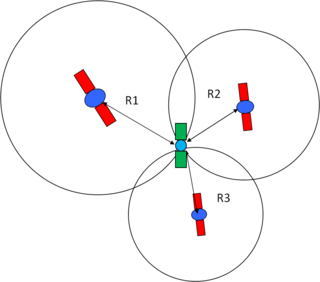
\includegraphics[width=5cm]{figures/gps_signals.png}
\caption{Semanlele radio GPS}
\label{fig:gps_signals}
\end{figure}

Pentru calculul locației curente se pleacă de la un fapt cunoscut, acela că receptorul se află fie pe suprafața Pământului, fie la o distanță mică de acesta (fie în aer sau în ocean).

Cunoscând acest fapt, estimarea locației la nivel de \textbf{latitudine} și \textbf{longitudine} se face cu doar \textbf{trei sateliți}. Sunt necesari trei sateliți pentru că unul din sateliți va juca rolul de satelit care oferă timpul de referință, iar ceilalți doi vor fi folosiți pentru a estima două sfere de probabilitate de apariție. Intersecția acelor două sfere va fi, în condițiile date, un punct sau maxim două puncte. Unul dintre acele puncte se va afla pe Pământ și celălalt în spațiu sau mult în interiorul Pământului (către centrul său). Receptorul GPS va ști să aleagă punctul aflat pe Pământ.\\

TODO: Modificare width imagine

TODO: Imagini cum se face 2D Fix (cu sferele)

TODO: Explicatii despre 3D Fix


\newpage
\bibliography{inside_nav_bib}
\bibliographystyle{unsrt}
\nocite{*}

\end{document}
